\documentclass[tikz]{standalone}
\usepackage{amsmath,amssymb,multirow}
\usetikzlibrary{shapes.misc, positioning,automata,arrows,calc,fit}
\tikzset{VertexStyle/.style = {draw,circle,thick,
		minimum size=1cm,
		font=\Large\bfseries},thick} 
\usepackage{braket}
\begin{document}
	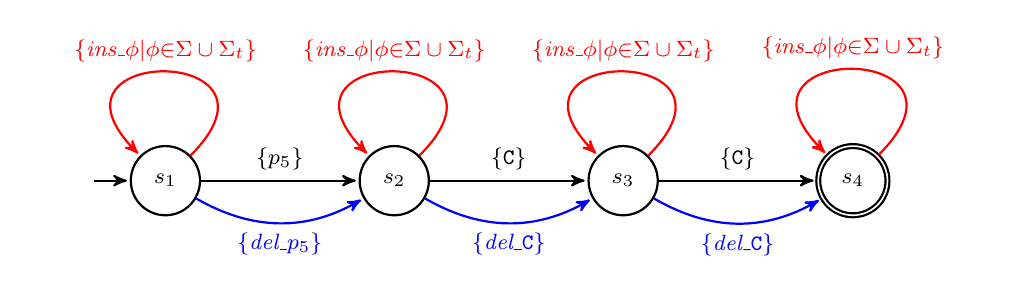
\begin{tikzpicture}[->,>=stealth',shorten >=1pt,thick,initial text=$ $,align=center,node distance=5mm,font=\footnotesize]
	\thickmuskip=0mu
	\node[state,initial] (SA) {$s_1$};
	\path (SA) edge[loop,red] node[midway,above] (W1) {$\{\textit{ins\_}\phi\;\;|\;\phi\in\Sigma\cup\Sigma_t\}$} (SA);
	\node[state,right =2cm of SA] (ST) {$s_2$};
	
	\path (ST) edge[loop,red] node[midway,above] (W2) {$\{\textit{ins\_}\phi\;\;|\;\phi\in\Sigma\cup\Sigma_t\}$} (ST);
	\draw[->] (SA) -- (ST) node[midway,above] {$ \{p_5\}$};
	\draw[->,blue] (SA) 
	edge [bend right] node[midway,below,sloped] {$\{\textit{del\_}p_5\}$} (ST)  ;
	
	\node[state,right=2cm of ST] (bot)  {$s_3$};
	\path (bot) edge[loop,red] node[midway,above]  {$\{\textit{ins\_}\phi\;\;|\;\phi\in\Sigma\cup\Sigma_t\}$} (bot);
	\draw[->] (ST) -- (bot) node[midway,above] {$ \{\texttt{C}\}$};
	\draw[->,blue] (ST) 
	edge [bend right] node[midway,below,sloped] {$\{\textit{del\_}\texttt{C}\}$} (bot)  ;
	
	\node[state,accepting,right=2cm of bot] (bot2)  {$s_4$};
	\path (bot2) edge[loop,red] node[midway,above]  {$\{\textit{ins\_}\phi\;\;|\;\phi\in\Sigma\cup\Sigma_t\}$} (bot2);
	\draw[->] (bot) -- (bot2) node[midway,above] {$ \{\texttt{C}\}$};
	\draw[->,blue] (bot) 
	edge [bend right] node[midway,below,sloped] {$\{\textit{del\_}\texttt{C}\}$} (bot2)  ;
	
	\end{tikzpicture}
\end{document}